\documentclass[12pt]{article}
\usepackage[english]{babel}
\usepackage{graphicx, amsmath, amsfonts, amsthm, mathtools, listings, color, caption, rotating, subfigure, fullpage, textcomp, enumitem, float, listings, MnSymbol, wasysym}

\lstset{
	language=R,
	keywordstyle=\bfseries\ttfamily\color[rgb]{0,0,1},
	identifierstyle=\ttfamily,
	commentstyle=\color[rgb]{0.133,0.545,0.133},
	stringstyle=\ttfamily\color[rgb]{0.627,0.126,0.941},
	showstringspaces=false,
	basicstyle=\tiny,
	numberstyle=\scriptsize,
	numbers=left,
	stepnumber=1,
	numbersep=10pt,
	tabsize=2,
	breaklines=true,
	breakatwhitespace=false,
	aboveskip={1.5\baselineskip},
  columns=fixed,
  upquote=true,
  extendedchars=true,
}

\begin{document}
\begin{center}
STA250, Final Project \\
Christopher Aden\\
December 9, 2013\
\end{center}

\section{Introduction}
We will revisit the probit regression model we introduced in Homework 4. 

The idea is simple: We observe an indicator function $y$ of an unobserved latent variable, $z$. To assess a relationship between $y$ and some covariates, we suppose that our $z$'s have a linear relationship to the covariates. If we impose normality on the latent variables, we can say that the probability of $y=1$ is $p = \Phi(X^T \beta)$. Probit regression is not a huge leap of the imagination if one is familiar with logistic regression--the difference is simply the choice of the link function. The goal is to estimate the influence of the covariates $\beta$ on the probability of observed $y$ being 1 or 0. Being Bayesians, we can also place prior belief on the values for $\beta$.

In the fourth homework assignment, we handled this problem through the magic of Gibbs sampling. This approach was very successful and very simple to implement. Since the conditionals could all be arrived at in closed form, standard R functions could be used, which meant sampling was somewhat fast. We also didn't have the problems Metropolis-Hastings has of rejecting outrageous proposals and staying too conservative, and we are not dependent on a smart choice for a proposal distribution.

These niceties are irrelevant if the samples from the Gibbs Sampler are very dependent. The purpose of this analysis will be to see whether the Metropolis-Hastings algorithm produces better samples than the Gibbs Sampler. We will also discuss certain properties of the MH Algorithm that are nicer than the Gibbs sampler. 

\section{Methodology}
This section will detail how to use Metropolis-Hastings to sample from the posterior of a Bayesian probit regression. The standard representation of Bayesian probit regression is the following model:
\begin{align*}
& \beta \sim N(\mu_0, \Sigma_0) \\
& y_{i} | \beta \sim \textrm{Bin}(1,\Phi(x_{i}^{T}\beta)) , \qquad i=1, \ldots, n,
\end{align*}
where $\Phi(x)$ is the CDF of the standard normal distribution. For tractability, assume the responses are conditionally independent given $\beta$.

Being unable to directly sample the posterior distribution acquired by a multivariate normal prior and a binomial likelihood, we are reduced to more computational methods--using either Gibbs sampling or Metropolis-Hastings. Assuming our likelihood and prior are specified as above, the posterior is thus
	\begin{align*}
	f(\underline{\beta} | \underline{y}) &\propto f(\underline{\beta}) \cdot \prod_{i=1}^n f(y_i | \beta) \quad \text{(by the cond. indep. of } y_i\text{ and Bayes' Theorem)} \\
	&= N(\mu_0, \Sigma_0) \cdot \prod_{i=1}^n \textrm{Bin}(1,\Phi((x_{i}^{T}\beta)))
	\end{align*}
This can be simplified further, but there's not much point. This distribution has no closed form in $\beta$. We cannot directly sample from it, so we apply Metropolis-Hastings.
	\begin{enumerate}
	\item[0] Specify a starting point for the Markov Chain, $\beta^0$.
	\end{enumerate}
	For each $i = 1, \dots, niter$:
	\begin{enumerate}[resume]
	\item Propose a new value, $\beta^*$, centered on the previous one, $\beta^i$.
	\item Compute the probability of the posterior at the candidate value $p(\beta^* | \underline{y})$, and the posterior at the current value $p(\beta^i | \underline{y})$. In R, just multiplying the prior by the likelihood, \texttt{dmvnorm} by \texttt{dbinom} is sufficient. For stability reasons, we work on the log scale, so we'll add the log-prior and the log-likelihood to get the log-posterior.
	\item Compute $\ln \alpha^* = \ln p(\beta^* | \underline{y}) - \ln p(\beta^i | \underline{y})$.
	\item Draw $U \sim U(0,1)$. If $\ln U \leq \ln \alpha^*$, set $\beta^{i+1} = \beta^*$. Else, $\beta^{i+1} = \beta^{i}$. The log scale will be equivalent with a greatly-reduced concern for numerical inaccuracy compared to the normal version.
	\item The vector $\beta^i$, $i=1, \dots, n$ represents \emph{dependent} draws from $p(\beta | \underline{y})$. 
	\end{enumerate}
	
The following summarizes some of the parameters I use to make the algorithm more efficient.
\begin{description}
\item[Starting Values:] To emulate the posterior mode with a completely uninformative prior, $\beta^0 = \hat{\beta}$, the MLE of the data. It can be shown that as the sample size increases, the effect of the prior diminishes for any non-degenerate prior, so for a large enough sample size and uninformative enough prior, the MLE will be close to the posterior mode. Using the MLE is a sensible choice if the sample size is large enough that the likelihood carries more weight in the posterior than the prior.

\item[Proposal Distribution] The proposal distribution is multivariate normal, centered on the previous value, with a covariance matrix $v^2 \Sigma$, where $v^2$ is a tuning parameter that changes to give a suitable acceptance rate. $\Sigma$ is the estimated covariance matrix using a Frequentist probit regression, which, for large enough sample size, closely models the structure of the posterior covariance. The normal was chosen because it is a symmetric distribution, which simplifies the math. The covariance was chosen to mimic the variance of the posterior with an uninformative prior (or large sample size).

\item[Tuning Process] It is possible that the proposal distribution does not have an appropriate variance. Too high a variance and we will propose improbable values, rejecting too often and ending up with lots of redundant draws. If the variance is too small, we will stay in relatively the same spot, not exploring the space effectively, accepting too often--we gain very little additional information on each draw. The solution to this problem is to keep track of our acceptance rates and make sure it stays within a good acceptance rate window. If the acceptance rate fell outside this band, I adjusted the proposal variance by a scalar factor of $v_i^{2} = \exp{(3 \cdot (\text{acceptance}-\text{ideal}))}$, where $v_i^2$ is the scalar proposed during this tuning period (the previous tuning period times the scaling factor). This worked for logistic regression, so we try it again here. I chose about 20\% as the ideal acceptance rate, based on simulation results on a multivariate normal. 

\item[Iterations] I spend very little time choosing a decent number of iterations. Millions of samples takes less than 10 minutes on my machine, with a retuning every thousand observations up to the burn-in.

\item[Burn-In] Like the number of iterations, the burn-in is somewhat of a non-issue. I chose to start at the MLE of the likelihood, which means my Markov Chain was pointed at the correct position from the very beginning. I could've chosen a very small burn-in if I wanted, but I also needed to adjust the proposal variance, so I set the burn-in to be more than $n/100$. If I could've adjusted the variance on-the-fly \emph{and} kept those draws instead of burning them, I could've made the burn-in period far less.
\end{description}

\section{Results}
The speed results are staggering, but must be taken with a grain of salt. 

First, we start with the run times. The Gibbs sampler was incredibly slow per iteration, compared to Metropolis Hastings. The need to sample the latent variables, $z$, meant that we had to do a lot more computational work, as well as require large amounts of memory. Metropolis-Hastings nicely avoids this problem by only needing to calculate the normal CDF of the covariates at each iteration of $\beta$. This negates needing truncated normal sampling at all! 

However... the Metropolis-Hastings suffers from a very high autocorrelation, because of how dependent the samples are (an inherent flaw in the method). While the Gibbs sampler is also correlated to the previous sample, it is not correlated to the same degree. As such, we require far fewer iterations before we are happy with our effective sample size. Looking at the autocorrelations on the first dataset ($n=10,000$), we can get an idea of how correlated the MH and Gibbs are, comparatively.

\begin{table}[H] \center
\begin{tabular}{ccc} \hline
$\beta_i$ & MH & Gibbs \\ \hline
1 & 0.932 & 0.599 \\ 
2 & 0.910 & 0.641 \\ 
3 & 0.927 & 0.680 \\ 
4 & 0.924 & 0.613 \\ 
5 & 0.930 & 0.795 \\ 
6 & 0.931 & 0.625 \\ 
7 & 0.923 & 0.673 \\ 
8 & 0.927 & 0.673 \\ \hline
\end{tabular}
\caption{Lag-1 Autocorrelations for Metropolis-Hastings versus Gibbs, Dataset 2, $n=10,000$}
\end{table}

How about the effective sample sizes for $3,000$ iterations?
\begin{table}[H] \center
\begin{tabular}{ccc} \hline
& MH & Gibbs \\ \hline
var1 & 90.16 & 608.07 \\ 
var2 & 98.67 & 637.55 \\ 
var3 & 113.54 & 388.06 \\ 
var4 & 130.65 & 568.59 \\ 
var5 & 95.11 & 279.89 \\ 
var6 & 102.70 & 570.49 \\ 
var7 & 117.18 & 438.30 \\ 
var8 & 119.51 & 432.54 \\ \hline
\end{tabular}
\caption{Effective Sample Size for MH and Gibbs samplers, $niter=3,000$, $n=10,000$.}
\end{table}

So the effective sample sizes range from 3 times better to as much as 7 times better for Gibbs versus Metropolis-Hastings. One suggestion is to just run the MH algorithm 7 times as long as the Gibbs sampler (or maybe a little more--for padding) to achieve a better effective sample size for the worst case variable. For larger data sets, this may make sense--the MH algorithm drastically outperforms Gibbs sampling as the cost of sampling the latent $z$'s increases. 

How does convergence look? On the $n=10,000$ dataset, we can run the Gibbs sampler with 3000 iterations and the Metropolis Hastings with $8 \cdot 3000 = 24,000$ iterations to compare.
\begin{figure}[H] \center
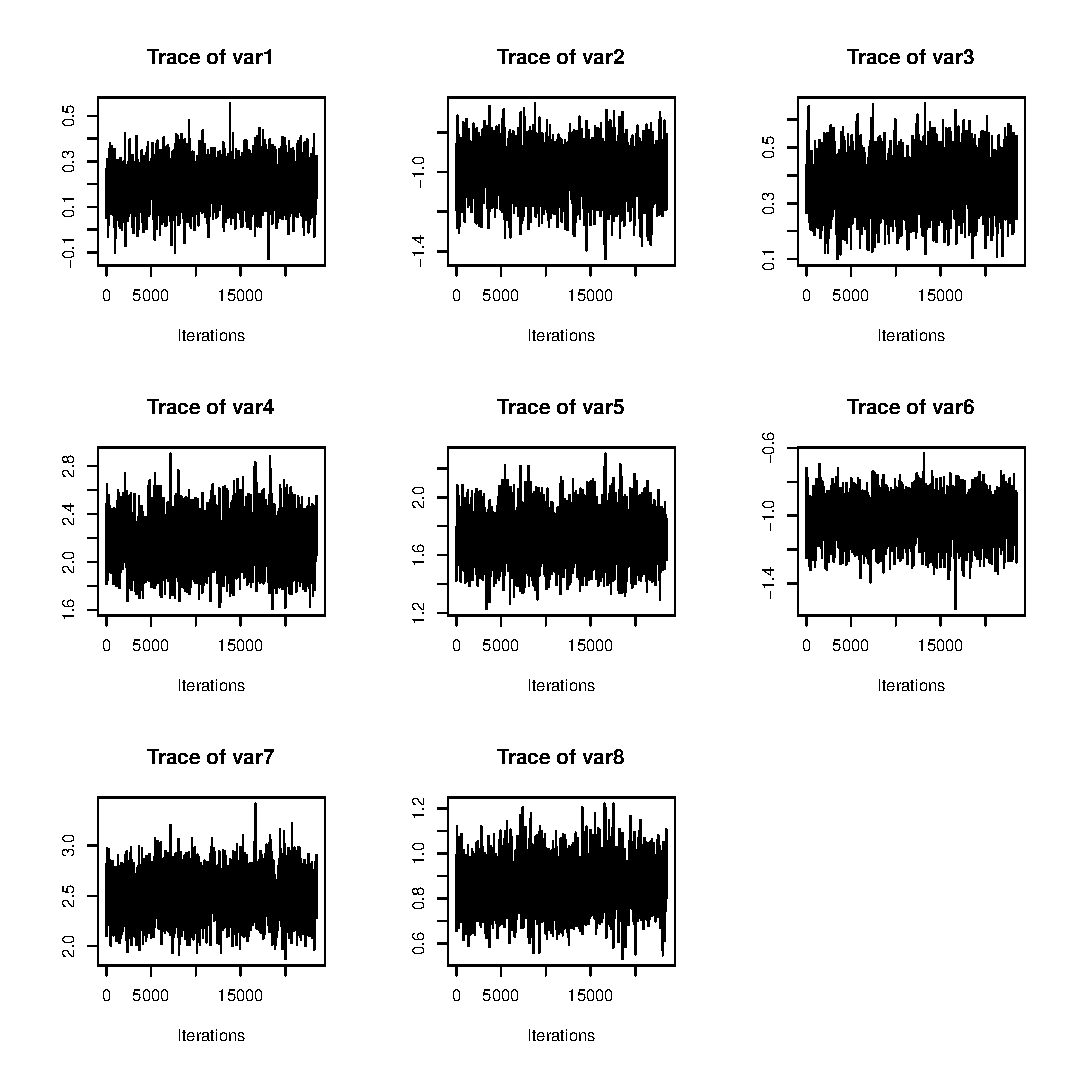
\includegraphics[scale=.45]{MH_Trace}
\caption{Trace plots for Metropois-Hastings, $niter=24,000$, $burnin=500$, $n=10,000$}
\end{figure}
\begin{figure}[H] \center
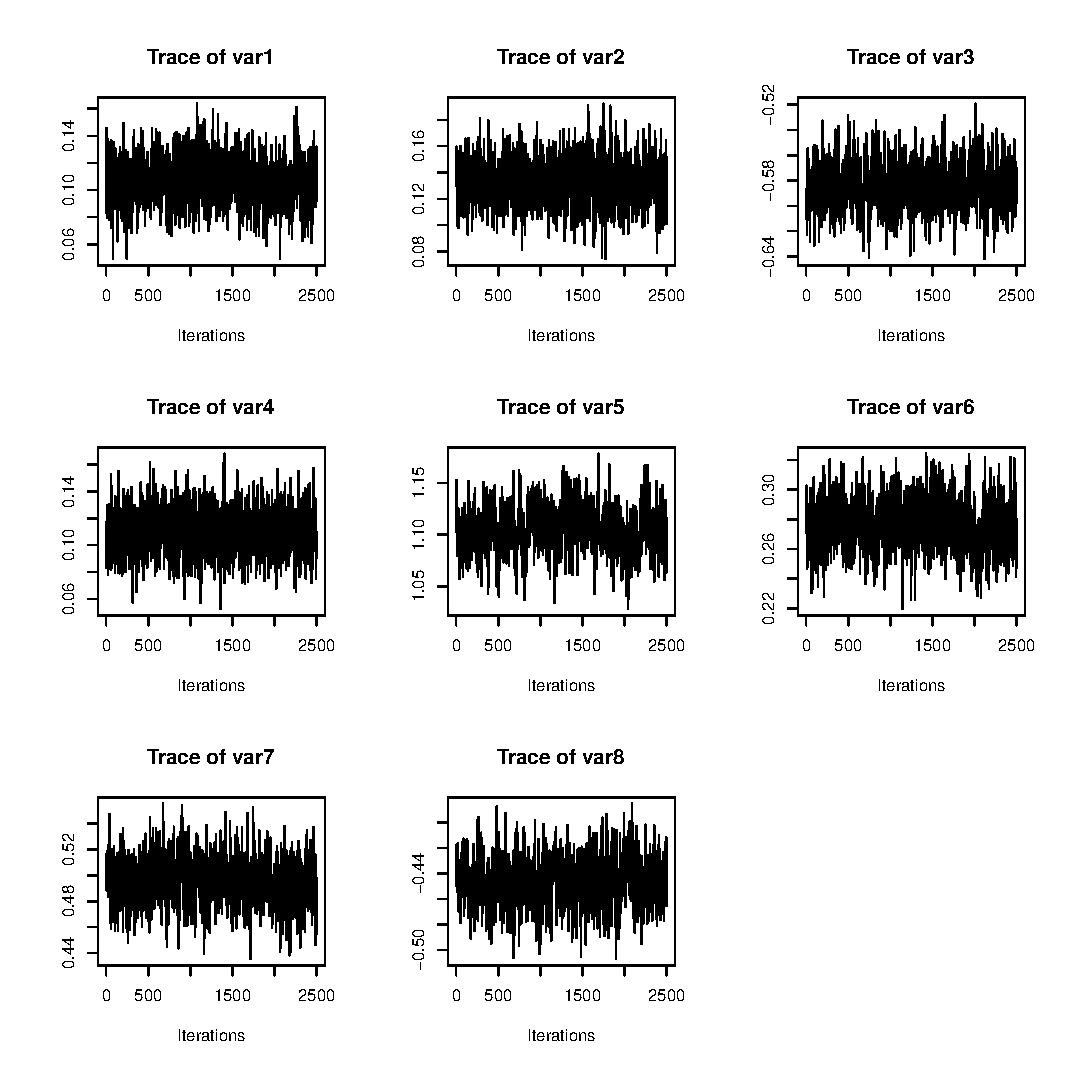
\includegraphics[scale=.45]{Gibbs_Trace}
\caption{Trace plots for Gibbs Sampler, $niter=3,000$, $burnin=500$, $n=10,000$}
\end{figure}
The convergence looks okay on both models, so let's go with these iterations. Now for a runtime comparison on the five datasets.

\begin{figure}[H] \center
\includegraphics[scale=.45]{Timings}
\caption{Runtimes on the five datasets, $3,000$ Gibbs samples, $24,000$ MH samples}
\end{figure}
The Metropolis-Hastings algorithm handily dominates Gibbs in all but the trivial case, despite having to generate eight times as many observations! Given that the Gibbs Sampler is sampling truncated normals--a step the MH algorithm is not doing--this shouldn't be too hard to believe. What is hard to believe are the actual run-times.

\begin{table}[H] \center
\begin{tabular}{ccc} \hline
& Gibbs Times & MH Times \\ \hline
1 & 8.42 & 22.43 \\ 
2 & 67.84 & 24.42 \\ 
3 & 661.15 & 23.91 \\ 
4 & 5285.45 & 23.64 \\ 
5 & 59380.66 & 24.52 \\ \hline
\end{tabular}
\caption{Run times for data sets of size $n = 10^3, \dots, 10^7$.}
\end{table}

It's as though the Metropolis-Hastings algorithm takes almost constant time, while the Gibbs sampler takes exponential time in $n$. The fact that MH took 24 seconds to calculate equivalent posterior draws from a dataset with $n=10,000,000$ and the Gibbs sampler took 17 hours should be enough information for us to strongly prefer using Metropolis-Hastings as the sample size increases.
\newpage
\section{Conclusions}
The Metropolis-Hastings algorithm handily manages to beat the runtime of the Gibbs sampler, even considering the very large handicap we pay for high autocorrelation. It's on this basis that makes a lot of sense to prefer MH over Gibbs when doing a Bayesian probit regression.

We pay a bit of an initial cost for having to generate so many more samples than the Gibbs sampler, as is manifested in the first dataset, but we \emph{very} quickly manage to overcome that initial cost, and for any non-trivially-sized data set, the MH algorithm is far faster. There is an exponential speedup for MH versus Gibbs if we're willing to draw more samples in exchange for a higher autocorrelation.

\section{Possible Extensions}
Writing the MH algorithm in C would've been a more appropriate comparison against the Gibbs sampler which had the advantage of using R constructs solely with very little overhead. Implementing my MH algorithm in C would've made for a more apt comparison.

From a more algorithmic side, Gibbs involved sampling a latent variable, and that was expensive. If the low autocorrelation of Gibbs could be combined with speed of Metropolis-Hastings, this would be an ideal. This could be achieved either through a less-dependent version of MH, or a version of Gibbs sampling that didn't involve having to sample from a truncated Normal distribution for the latent variables.

\section{Self-Criticisms}
The Metropolis-Hastings could've been written on the GPU very easily. It is a far more tractable GPU problem than the Gibbs sampler which involves generating truncated normals. For the MH algorithm, all we have to do is calculate a normal CDF at each iteration, as well as evaluate a binomial PDF. This is an ``embarassingly parallel'' problem. I could imagine the run time would be phenomenal compared to a pure-CPU implementation.

I wish I had the time to play around with alternative proposal distributions. The Metropolis algorithm was thoroughly bothered by high autocorrelation. Potentially, a smarter proposal could've made for more efficient sampling. It's also possible that alternative MCMC algorithms would've been good to research. If Gibbs was more efficient, it could've been a smart choice (it was very easy to write).

\newpage
\section{Appendix}
\subsection*{R Source Code}
Helper\_functions is a script containing the majority of the algorithms I used to do Bayesian probit regression. It contains basic functions, as well as my Metropolis Hastings implementation and Gibbs sampler implementation.
\lstinputlisting{"helper_functions.R"}

\newpage
Probit\_mcmc handles the work of calling the simulated data sets and running the Gibbs and MH samplers over them. It also deals with saving and plotting.
\lstinputlisting{"probit_mcmc.R"}
\end{document} 